\documentclass[conference]{IEEEtran}
\IEEEoverridecommandlockouts
\renewcommand{\refname}{Bibliografía}
% The preceding line is only needed to identify funding in the first footnote. If that is unneeded, please comment it out.
\usepackage{cite}
\usepackage{amsmath,amssymb,amsfonts}
\usepackage{algorithmic}
\usepackage{graphicx}
\usepackage{textcomp}
\usepackage{xcolor}
\usepackage{url}
\usepackage{upgreek}
\usepackage{amssymb}
\usepackage{verbatim}
\def\BibTeX{{\rm B\kern-.05em{\sc i\kern-.025em b}\kern-.08em
    T\kern-.1667em\lower.7ex\hbox{E}\kern-.125emX}}
\begin{document}

\title{Proyecto 3\\
{\footnotesize \textsuperscript{}IC3002 - Análisis de Algoritmos}
{\footnotesize \textsuperscript{}Profe.: Yuen Law Wan}
{\footnotesize \textsuperscript{}I Semestre 2020}
}

\author{\IEEEauthorblockN{Joseph Tenorio Pereira}
\IEEEauthorblockA{\textit{2019064588} \\
}
\and
\IEEEauthorblockN{Jose Pablo Muñoz Montero}
\IEEEauthorblockA{\textit{2019061904} \\
}
}

\maketitle

\begin{abstract}
The following documentation revolves around the desing, analysis, and \textit{Python} implementation of a Genetic Algorithm whose purpose is to produce simulated robots capable of solving a given maze. The aforementioned robots are to have certain simulated properties suchs as hardware, cost and behaviour, and it is through these characteristics that the Genetic Algorithm is expected to generate better robots with each iteration. All parts of the creation of a Genetic Algorithm will be discussed as part of the design, that includes chromosome and adaptability function definition, selection, mutation and crossover. Aditionally, the behaviour property is to be dictated by a Markov Chain representation, so the combination of Genetic Algorithms and Markov Chains is briefly covered. Finally, results of the implementation will be shown, emphasizing the difference between the firsts and lasts generations, and conclusions will be drawn.
\end{abstract}

\section{Introducción}

Los algoritmos genéticos se entienden, según \cite{b1}, como un tipo de algoritmo evolutivo en el que representaciones de posibles soluciones, llamadas genes o cromosomas, son puestos a prueba, cruzados y mutados con el fin de llegar a genes mejor adaptados, es decir, soluciones óptimas. El cruce y selección de genes es hecho con base en la selección natural biológica, de hecho, los algoritmos genéticos en general están inspirados en dicho mecanismo evolutivo. Otro ejemplo de lo anterior es la introducción de mutaciones a los genes, es decir, cambiar aleatoriamente los valores de los mismos, de modo que  se cuente con un minímo de aleatoriedad en el algoritmo. Los componentes más importantes del diseño de un algoritmo genético suelen ser la definición, selección y cruce de los cromosomas, y son precisamente estos componentes del algoritmo los que seran discutidos en el presente documento. Cabe señalar que la función de adaptabilidad del algoritmo, aquella formula por medio de la cual se determinan cuáles soluciones son más deseables que otras, es también discutida durante el proyecto. 

Otro concepto a tener en cuenta en el presente proyecto es el de cadenas de Markov, las cuáles de acuerdo a \cite{b2} se suelen explicar como un conjunto de propiedades juntadas y representadas como un estado (aquí llamados "nodos") y las probabilidades de que el proceso representado por la cadena pase de un estado a cualquier otro (aquí llamados "arcos"). Cabe resaltar que las cadenas de Markov son una forma de representar los procesos de Markov y estos últimos tienen la propiedad fundamental de que la probabilidad de pasar de un estado a otro depende únicamente del estado actual. Tomando en cuenta lo anterior, es posible describir y estimar una predicción de una amplia gama de comportamientos por medio de cadenas de Markov, ya que es posible representar dicho comportamiento como una serie de recorridos a lo largo del tiempo entre los estados, donde la elección del siguiente estado es dictada por la probabilidad entre dicho estado y el actual.

El presente proyecto busca diseñar un algoritmo genético capaz de producir robots eficientes en la resolución de un laberinto dado. Para ello se requiere, además del algoritmo en sí, la completa simulación del proceso de los robots resolviendo el laberinto. Esto último incluye la representación del laberinto dentro del programa con sus respectivos tipos de terreno, de los robots por medio de las características de cámara (permite ver casillas alrededor), motor (permite atraviesar o no ciertos terrenos), batería (determina qué tanto se puede mover el robot), comportamiento, costo (resumen de la calidad del equipo del robot) y el propio intento de resolución del algoritmo. Como parte del diseño del algoritmo se definirán los cromosomas de los robots con base en las propiedades antes listadas, lo cual incluirá la representación de una cadena de Markov en los cromosomas, ya que se espera también diseñar cadenas de Markov capaces de dictar el comportamiento de los robots durante su intento de resolver el laberinto. Otro objetivo a destacar del presente proyecto es la confección de una función de adaptabilidad dentro de la selección algoritmo capaz de definir lo que se considera una solución óptima, es decir, un robot eficiente en la resolución del laberinto, basada en los parámetros de recorrido, costo y tiempo tomado por parte del robot. Claramente, también se busca la programación de las demás partes del algoritmo genético, específicamente, el cruce y mutación de los cromosomas de modo que se creen las subsecuentes generaciones hasta que se alcance la optimización deseada. Finalmente, se apunta a implementar todo lo anterior en un programa de \textit{Python} que además muestre ciertos aspectos del algoritmo, tales como historial de los cruces realizado y optimización de los robots en las generaciones dadas, de manera amigable para el usuario, por medio de una interfaz gráfica a diseñar.

\section{Trabajo Relacionado}
Los algoritmos genéticos pueden ser empleados para encontrar soluciones óptimas a una amplia gama de problemas y a la vez no requerir mucha complejidad de programación en su implementación. Lo anterior se ve evidenciado por el trabajo realizado por \cite{b3}, en donde se programa en \textit{Python} un breve y simple algoritmo genético cuyo objetivo es producir \textit{smart boxes} con un comportamiento que los haga capaces de ir del borde de un rectángulo a otro evitando obstáculos lineales. Por medio de la ejecución de dicho programa se evidencia la mejora general entre generaciones, ya que las \textit{smart boxes} se acercan cada vez más al otro lado del rectángulo sin quedar atascadas en los obstáculos. Lo anterior se asemeja mucho a uno de los objetivos del presente proyecto, es decir, se busca que el algoritmo sea capaz de trabajar con cromosomas que representan el comportamiento de un objeto navegante. No obstante, dicho cromosoma se representa por medio de una lista de movimientos con aceleración aleatoria, mientras que el programa aquí diseñado busca representar una cadena de Markov en su lugar.

Por otro lado, las cadenas de Markov también son usadas para representar una amplia de gama de comportamientos. Una de las muchas aplicaciones de dichas representaciones es la encontrada en las cadenas de Markov Monte Carlo (\textit{Markov Chain Monte Carlo, MCMC}), en las cuales se emplea un método de Monte Carlo que toma muestras de los estados de una cadena de Markov para aproximar una función de distribución de probabilidad. En \cite{b4} se puede encontrar una implementación de MCMC en \textit{Python}, la cual, de manera similar al presente proyecto, se encuentra el problema de la representación de cadenas de Markov en \textit{Python}, lo cual se acaba solucinando por medio de la librería de  \textit{PyMC3}.  

\section{Metodología}

Primeramente, es necesario definir las estructuras usadas en la programación del algoritmo genético. El labarinto empleado corresponde a una matriz 20 x 20, la cual almacena enteros 


\section{Análisis de resultados}


\begin{figure}[htbp]
\centerline{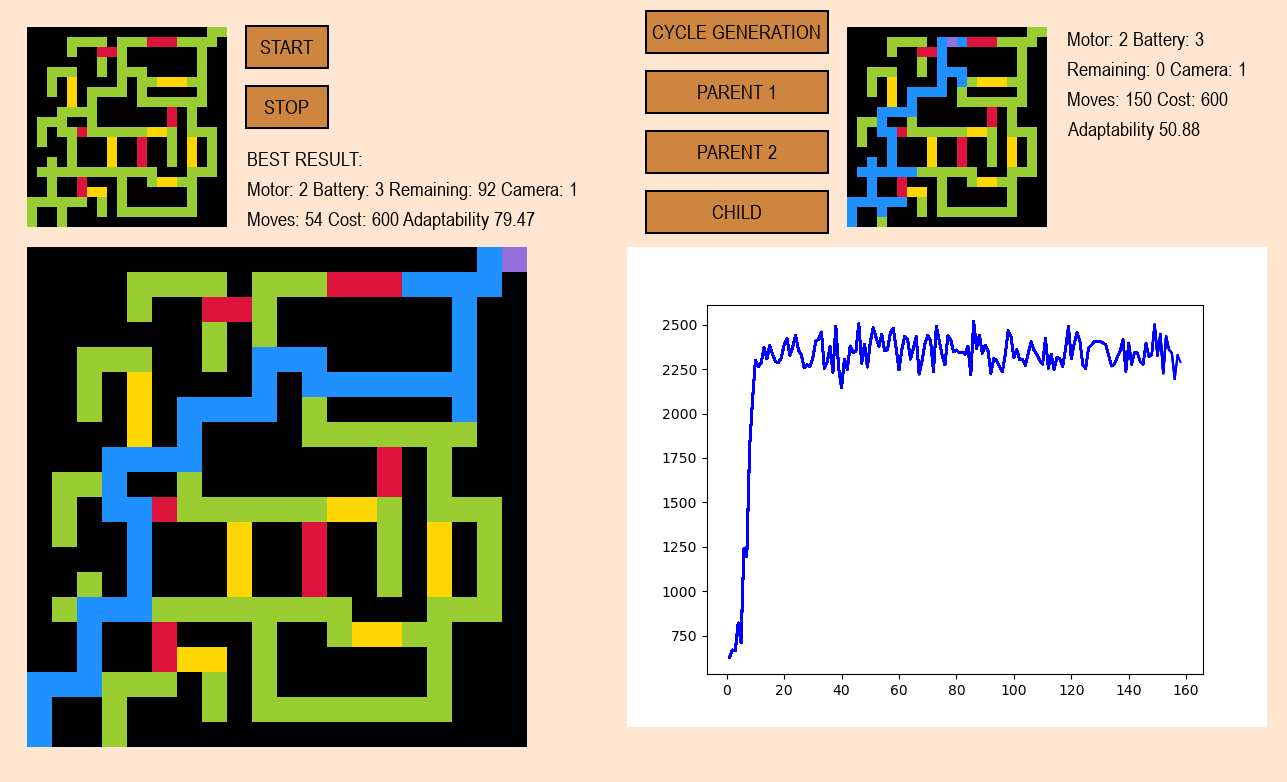
\includegraphics[scale=0.68]{Resultado2.png}}
\caption{Imagen a renderizar. Las fuentes de luz se circulan en rojo. Las superficies se resaltan en azul las especulares, blanco las transparentes y verde las regulares}
\label{Imagen de referencia}
\end{figure}


\begin{figure}[htbp]
\centerline{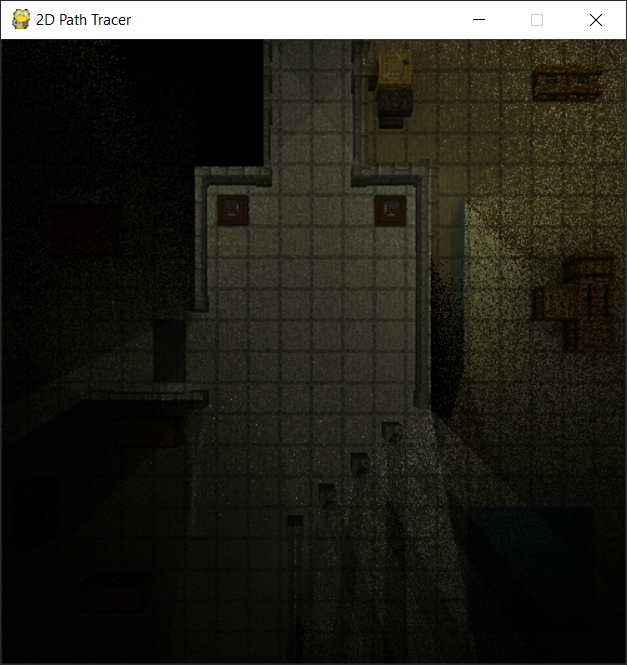
\includegraphics[scale=0.68]{Resultado1.png}}
\caption{Renderización completa con 50 muestras. Tiempo de ejecución: 16 minutos con 20 segundos.}
\label{50 muestras completo}
\end{figure}


\section{Conclusión}


\section{Acceso al proyecto}
El repositorio de GitHub en el cual se ubican todos los archivos empleados para el desarrollo de este proyecto puede ser accesado mediante el siguiente link: \url{https://github.com/TilapiaBoi/AnalisisPRY3}

\begin{thebibliography}{00}
\bibitem{b1} W. Hosch, \textit{Genetic algorithm}. Encyclopædia Britannica. n.d. Accesed on: Jul. 30, 2020. [Online]. Available: \url{https://www.britannica.com/technology/genetic-algorithm}
\bibitem{b2} S. Jaiswal, \textit{Markov Chains in Python: Beginner Tutorial}. Dec. 31, 2019. Accesed on: Jul 29, 2020. [Online]. Available: \url{https://www.datacamp.com/community/tutorials/markov-chains-python-tutorial}
\bibitem{b3} B. Unutmaz, \textit{Smart Boxes - Python AI Genetic Algorithm ( with Source Code )}, Sep. 25, 2019. Accessed on: Jul. 29,2020. [Video file]. Available: \url{ https://www.youtube.com/watch?v=GiaSEsZjWNc}
\bibitem{b4} W. Koehrsen, \textit{Markov Chain Monte Carlo in Python}. Feb. 9, 2018. Accesed on: Jul. 28, 2020. [Online]. Available:\url{https://towardsdatascience.com/markov-chain-monte-carlo-in-python-44f7e609be98}
\end{thebibliography}
\end{document}